\chapter{Arhitektura i dizajn sustava}
		

		 Stil višeslojne arhitekture odjeljuje cjelovite komponente i te princip oblikovanja podijeli pa vladaj može preuzeti već postojeću podjelu. Troslojni stil arhitekture je prilagođen za jednostavne web aplikacije i mi ćemo ga koristiti za izradu naše aplikacije.
		 
		Arhitektura koju smo izabrali temelji se na principu oblikovanja podijeli pa vladaj. Tim principom smo uspjeli postići da odvojeni manji timovi unutar našeg tima rade na manjim problemima čime smo omogućili specijalizaciju. Takva podjela omogućuje efikasniji rad tima.
		
		\vspace{5mm}
		\noindent Arhitektura se sastoji od tri sloja:
		\begin{packed_enum}
			\item  podatkovni sloj
		
			\item  sloj poslovne logike
		
			\item  korisnički ili prezentacijski sloj
		\end{packed_enum}
	
	Podatkovni sloj je sloj za pohranu podataka u bazu ili datotečni sustav. U našoj aplikaciji koristit će se relacijska baza podataka, a odabrani jezik je SQL te razvojno okruženje PosgreSQL, pgAdmin . Također u početcima izrade aplikacije drugi slojevi će moći koristiti privremenu H2 bazu podataka pisanu u programskom jeziku Java u razvojom okruženju IntelliJIDEA.
	
	Sloj poslovne logike je sloj s implementacijom poslovnih procesa i izračuna. Kod web aplikacija ovaj sloj je podržan od strane web poslužitelja ili aplikacijskog poslužitelja. Ovaj sloj obrađuje i generira dinamički sadržaj koji prosljeđuje sljedećem sloju.
	
	Korisnički ili prezentacijski sloj je sloj s korisničkim sučeljem. Ovaj sloj kod web aplikacija se sastoji od web poslužitelja koji isporučuje statički i dinamički sadržaj, a sadržaj web stranice prikazuje web preglednik. Web poslužitelj to izvršava pomoću mrežnih protokola, a to su HTTP protokoli. Korisnik pomoću ovog sloja šalje upite i naredbe sloju poslovne logike koji ih obrađuje, te također pregledava sadržaj koji mu pruža sloj poslovne logike.

		Za razvoj naše aplikacije koristimo radni okvir Java Spring Boot. Pri korištenju tog radnog okvira potrebno je dodati još dodatnih slojeva u arhitekturu pri čemu se klijenstka i poslužiteljska strana mogu organizirati u više slojeva, ali ne utječu na organizaciju tima po glavna tri sloja.
		
		\vspace{5mm}
		\noindent Višeslojna se arhitektura u tom slučaju dijeli na šest slojeva:
		\begin{packed_enum}
			\item  sloj korisničke strane
		
			\item  sloj nadglednika
	
			\item  sloj usluge
		
			\item  sloj domene
		
			\item  sloj za pristup podatcima
		
			\item  sloj baze podataka
		\end{packed_enum}
		
	Sloj korisničke strane implementiran je u JavaScriptu, koristi React koji omogućuje prikaz korisničkog sučelja,a korištena paltforma je Microsoft visual studio.
	
	Sloj nadglednika povezuje korisničku stranu s poslužiteljskom stranom. Implementiran je u jeziku Java na platformi IntelliJIDEA.
	
	Sloj usluge obavlja svu poslovnu logiku i potrebne izračune. Implementiran je u jeziku Java na platformi IntelliJIDEA.
	
	Sloj domene ima razrađeni model podataka domene. Implementiran je u jeziku Java na platformi IntelliJIDEA.
	
	Sloj za pristup podatcima je sloj koji omogućuje spremanje i dohvat podataka iz određene baze podataka te razmjenu tih podataka sa slojem domene. Implementiran je u jeziku Java na platformi IntelliJIDEA.
	
	 Sloj baze podataka omogućuje pohranu podataka u relacijsku bazu ili H2 bazu. Za relacijsku bazu koriste se PostgreSQL i pgAdmin, a za H2 bazu koristi se Java na platformi IntelliJIDEA.
	
		

		

				
		\section{Baza podataka}
			
	  Naš sustav zahtijeva pohranu puno podataka, stoga je bilo potrebno izraditi relacijsku bazu podataka koju bi mogli koristiti za te potrebe. Baza nam je potrebna također za izmjenu i dohvat podataka za daljnju obradu te nam omogućava trajno čuvanje podataka. U ovoj ranijoj fazi izgradnje programske potpore za naš sustav odlučili smo se za jednostavniju verziju baze podataka H2 koja pohranjuje podatke u memoriju računala na kojemu je program pokrenut. U kasnijim fazama razvoja potpore ćemo se povezati na trajnu bazu podataka. Baza podataka koja nam je potrebna za naš sustav sastoji se od sljedećih entiteta:
		\begin{itemize}
			\item user
			\item address
			\item city
			\item role
			\item category
			\item ad
			\item condition
			\item message
			\item usersPrefersCategory
			\item adInCategory
			
		
		\end{itemize}
		
			\subsection{Opis tablica}
			
				\textbf{User	}
				Ovaj entitet modelira korisnika naše aplikacije. Entitet sadrži sljedeće atribute: idUser, userName, email, password, name, surname, idAdress i idRole. Atribut surname je opcionalan. Ovaj entitet je u vezi Many-to-One s entitetom Adress preko entiteta idAddress te u vezi Many-to-One s entitetom Role preko atributa idRole.
				
				\begin{longtabu} to \textwidth {|X[6, l]|X[6, l]|X[20, l]|}
					
					\hline \multicolumn{3}{|c|}{\textbf{User}}	 \\[3pt] \hline
					\endfirsthead
					
					\hline \multicolumn{3}{|c|}{\textbf{User}}	 \\[3pt] \hline
					\endhead
					
					\hline 
					\endlastfoot
					
					\cellcolor{LightGreen}\textbf{idUser} & INT	&  	Identifikacijski broj korisnika 	\\ \hline
					userName & VARCHAR	&  	Korisničko ime 	\\ \hline
					email	& VARCHAR &   Mail adresa korisnika	\\ \hline 
					password & VARCHAR & Lozinka korisnika  \\ \hline 
					name & VARCHAR	&  	Ime korisnika	\\ \hline 
					surname & VARCHAR	&  	Prezime korisnika	\\ \hline 
					
					\cellcolor{LightBlue}\textit{ idAdress}	& INT & Identifikacijski broj adrese korisnika   	\\ \hline 
					\cellcolor{LightBlue} \textit{ idRole}	& INT & Identifikacijski broj uloge korisnika   	\\ \hline 
					
					
				\end{longtabu}
				
				
				\textbf{Address		}
				Ovaj entitet predstavlja adresu našega korisnika. Sadrži atribute: idAddress, street, number, latitude, longitude i postalCode. Ovaj entitet u vezi je Many-to-One s entitetom City preko atributa postalCode.
				
				
				\begin{longtabu} to \textwidth {|X[6, l]|X[6, l]|X[20, l]|}
					
					\hline \multicolumn{3}{|c|}{\textbf{Address}}	 \\[3pt] \hline
					\endfirsthead
					
					\hline \multicolumn{3}{|c|}{\textbf{Address}}	 \\[3pt] \hline
					\endhead
					
					\hline 
					\endlastfoot
					
					\cellcolor{LightGreen}\textbf{idAddress}  & INT	&  	Identifikacijski broj adrese	\\ \hline
					street & VARCHAR	&  	Ulica lokacije 	\\ \hline
					number	& INT &  Kućni broj lokacije	\\ \hline 
					latitude & VARCHAR & Geografska širina lokacije \\ \hline 
					longitude & VARCHAR	&  Geografska duljina lokacije	\\ \hline 
					
					\cellcolor{LightBlue} \textit{  postalCode}	& INT & Poštanski broj mjesta u kojemu se nalazi \newline lokacija	\\ \hline  
					
					
				\end{longtabu}
				
				
			\textbf{City		}
				Ovaj entitet predstavlja grad unutar kojega živi naš korisnik. Sadrži atribute postalCode i cityName. 
				
				\begin{longtabu} to \textwidth {|X[6, l]|X[6, l]|X[20, l]|}
					
					\hline \multicolumn{3}{|c|}{\textbf{City}}	 \\[3pt] \hline
					\endfirsthead
					
					\hline \multicolumn{3}{|c|}{\textbf{City}}	 \\[3pt] \hline
					\endhead
					
					\hline 
					\endlastfoot
					
					\cellcolor{LightGreen} \textbf{postalCode} & INT	&  	Poštanski broj mjesta u kojemu se nalazi \newline lokacija	\\ \hline
					cityName & VARCHAR	&  Naziv grada u kojemu se nalazi lokacija 	\\ \hline			
					
				\end{longtabu}
				
				
				\textbf{Role		}
				Ovaj entitet predstavlja ulogu koju naš korisnik može imati. Sadrži atribute idRole i roleName.
				
				
				\begin{longtabu} to \textwidth {|X[6, l]|X[6, l]|X[20, l]|}
					
					\hline \multicolumn{3}{|c|}{\textbf{Role}}	 \\[3pt] \hline
					\endfirsthead
					
					\hline \multicolumn{3}{|c|}{\textbf{Role}}	 \\[3pt] \hline
					\endhead
					
					\hline 
					\endlastfoot
					
					\cellcolor{LightGreen} \textbf{idRole} & INT	&  	Identifikacijski broj uloge koju korisnik može \newline imati u sustavu	\\ \hline
					roleName & VARCHAR	&  	Naziv uloge  	\\ \hline
					
					
					
				\end{longtabu}
				
				
				\textbf{Category		}
				Ovaj entitet predstavlja kategoriju koju naš oglas može imati. Sadrži atribute idCategory te categoryName.
				
				
				\begin{longtabu} to \textwidth {|X[6, l]|X[6, l]|X[20, l]|}
					
					\hline \multicolumn{3}{|c|}{\textbf{Category}}	 \\[3pt] \hline
					\endfirsthead
					
					\hline \multicolumn{3}{|c|}{\textbf{Category}}	 \\[3pt] \hline
					\endhead
					
					\hline 
					\endlastfoot
					
					\cellcolor{LightGreen} \textbf{idCategory} & INT	&  	Identifikacijski broj kategorije	\\ \hline
					categoryName & VARCHAR	&  Naziv kategorije 	\\ \hline
										
				\end{longtabu}
		
		
		
		
				
				\textbf{Ad		}
				Ovaj entitet modelira oglas koji povezuje one koji žele prodati proizvod i one koji žele kupiti proizvod. Entitet sadrži atribute: idAd, caption, image, description, price, discount, timeOfAddition, timeOfExpiration, IdUserSeller, IdUserBuyer i  idCondition. Ovaj entitet u vezi je One-To-One s entitetom Condition preko idCondition, u vezi Many-to-One sa entitetom User preko atributa IdUserSeller te i preko atributa IdUserBuyer.
\begin{longtabu} to \textwidth {|X[10, l]|X[6, l]|X[20, l]|}
					
					\hline \multicolumn{3}{|c|}{\textbf{Ad}}	 \\[3pt] \hline
					\endfirsthead
					
					\hline \multicolumn{3}{|c|}{\textbf{Ad}}	 \\[3pt] \hline
					\endhead
					
					\hline 
					\endlastfoot
					
					\cellcolor{LightGreen} \textbf{idAd} & INT	&  	Identifikacijski broj oglasa	\\ \hline
					caption & VARCHAR	&  	Naslov oglasa 	\\ \hline
					image	& LONGBLOB &  Slika oglasa	\\ \hline 
					description & VARCHAR & Opis oglasa \\ \hline 
					price & DECIMAL	&  Cijena oglasa	\\ \hline 
					discount & INT	&  Popust koji se ostvaruje	\\ \hline 
					timeOfAddition & DATETIME	&  Vrijeme postavljanja oglasa	\\ \hline 
					timeOfExpiration & DATETIME	&  Vrijeme trajanja oglasa	\\ \hline 
					
					\cellcolor{LightBlue} \textit{  IdUserSeller}	& INT & Identifikacijski broj korisnila koji je \newline objavio oglas	\\ \hline  
					\cellcolor{LightBlue} \textit{  IdUserBuyer}	& INT & Identifikacijski broj korisnila koji je \newline kupio preko oglas	\\ \hline  
					\cellcolor{LightBlue} \textit{  idCondition}	& INT & Identifikacijski broj stanja oglasa\\ \hline  
					
					
				\end{longtabu}
				
				
				
				
				\textbf{Condition 		}
				Ovaj entitet predstavlja  stanje u kojemu se nalazi oglas. Entitet sadrži atribute: idCondition i conditionName.
				
				\begin{longtabu} to \textwidth {|X[8, l]|X[6, l]|X[20, l]|}
					
					\hline \multicolumn{3}{|c|}{\textbf{Condition}}	 \\[3pt] \hline
					\endfirsthead
					
					\hline \multicolumn{3}{|c|}{\textbf{Condition}}	 \\[3pt] \hline
					\endhead
					
					\hline 
					\endlastfoot
					
					\cellcolor{LightGreen} \textbf{idCondition} & INT	&  	Identifikacijski broj stanja	\\ \hline
					conditionName & VARCHAR	&  	Naziv stanja \\ \hline
					
					
				\end{longtabu}
				
				
				
				
				\textbf{Message 		}
				Ovaj entitet modelira poruke koje izmjenuju kupac i prodavač. Entitet sadrži atribute: idMessage, text, time, idUserRecieved i idUserSent. Entitet je u vezi Many-to-One sa entitetom User preko atributa idUserSent i atributa idUserRecieved.
				
				
				\begin{longtabu} to \textwidth {|X[8, l]|X[6, l]|X[20, l]|}
					
					\hline \multicolumn{3}{|c|}{\textbf{Message}}	 \\[3pt] \hline
					\endfirsthead
					
					\hline \multicolumn{3}{|c|}{\textbf{Message}}	 \\[3pt] \hline
					\endhead
					
					\hline 
					\endlastfoot
					
					\cellcolor{LightGreen} \textbf{idMessage} & INT	&  	Identifikacijski broj poruke\\ \hline
					text & VARCHAR	&  	Tekst poruke 	\\ \hline
					time	& DATETIME &  Vrijeme poruke	\\ \hline 
					
					\cellcolor{LightBlue} \textit{  idUserRecieved}	& INT & Identifikacijski broj korisnika koji je dobio \newline poruku	\\ \hline  
					\cellcolor{LightBlue} \textit{  idUserSent}	& INT & Identifikacijski broj korisnika koji je poslao \newline poruku	\\ \hline  
					
					
				\end{longtabu}
				
				
				\textbf{UsersPrefersCategory 		}
				Ovaj entitet sadrži podatke koji nam govore koje su korisniku najdraže kategorije oglasa. Entitet sadrži atribute: idUser i idCategory. Entitet je u vezi Many-to-Many sa entitetom User preko atributa idUser te je u vezi Many-to-Many sa entitetom Category preko atributa idCategory.
				
				\begin{longtabu} to \textwidth {|X[6, l]|X[6, l]|X[20, l]|}
					
					\hline \multicolumn{3}{|c|}{\textbf{UsersPrefersCategory}}	 \\[3pt] \hline
					\endfirsthead
					
					\hline \multicolumn{3}{|c|}{\textbf{UsersPrefersCategory}}	 \\[3pt] \hline
					\endhead
					
					\hline 
					\endlastfoot
					
					\cellcolor{LightGreen} \textbf{idUser} & INT	&  	Identifikacijski broj korisnika 	\\ \hline
					
					\cellcolor{LightBlue} \textit{  idCategory}	& INT & Identifikacijski broj kategorija koje korisnik \newline preferira	\\ \hline  
					
					
				\end{longtabu}
				
				
				
				\textbf{AdInCategory 		}
				Ovaj entitet sadrži podatke koji nam govore koje sve kategorije mogu biti oglasi. Entitet sadrži atribute: idAd i idCategory. Entitet je u vezi Many-to-Many sa entitetom Ad preko atributa idAd te je u vezi Many-to-Many sa entitetom Category preko atributa idCategory.
				
				
				\begin{longtabu} to \textwidth {|X[6, l]|X[6, l]|X[20, l]|}
					
					\hline \multicolumn{3}{|c|}{\textbf{AdInCategory}}	 \\[3pt] \hline
					\endfirsthead
					
					\hline \multicolumn{3}{|c|}{\textbf{AdInCategory}}	 \\[3pt] \hline
					\endhead
					
					\hline 
					\endlastfoot
					
					\cellcolor{LightGreen} \textbf{idAd} & INT	&  	Identifikacijski broj oglasa	\\ \hline
					
					\cellcolor{LightBlue} \textit{  idCategory}	& INT & Identifikacijski broj kategorije oglasa	\\ \hline  
					
					
				\end{longtabu}
				
			
			\subsection{Dijagram baze podataka}
			
				\begin{figure}[H]
			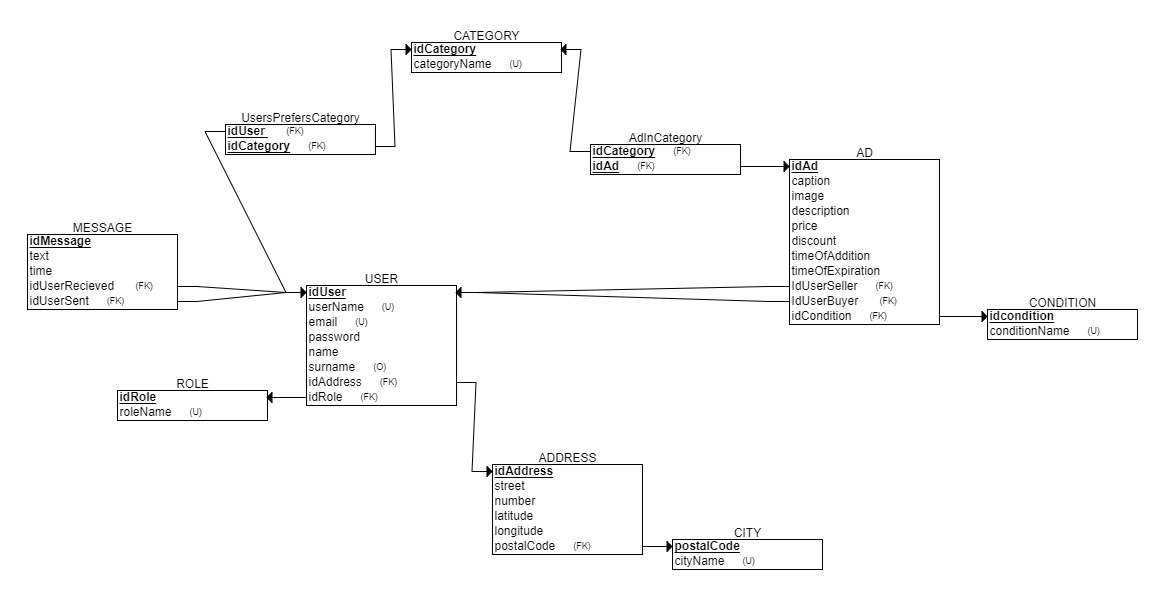
\includegraphics[scale=0.4]{slike/DijagramBaze.PNG} %veličina slike u odnosu na originalnu datoteku i pozicija slike
			\centering
			\caption{E-R dijagram baze podataka}
			\label{fig:dijagramBaze}
		\end{figure}
			\eject
			
		\section{Dijagram razreda}
		
		Na slikama su prikazani razredi koji pripadaju backend dijelu arhitekture. Prva slika prikazuje razred UserController i AuthController koji nasljeđuju razred Contoller. Metode implementirane u tim razredima manipuliraju s DTO(Data transfer object) , a oni su dohvaćeni pomoću metoda implementiranih u Model razredima.
		
			
			\begin{figure}[H]
				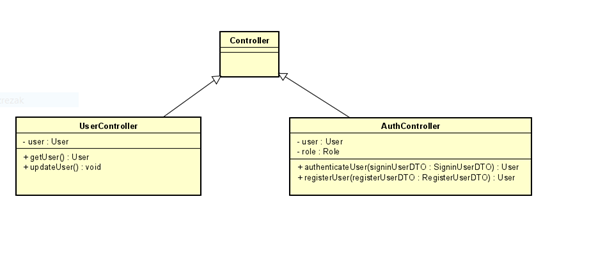
\includegraphics[scale=1]{slike/DijagramRazredaC.PNG} %veličina slike u odnosu na originalnu datoteku i pozicija slike
				\centering
				\caption{Dijagram razreda - Controllers}
				\label{fig:dijagramRazredaC}
			\end{figure}
		
			\begin{figure}[H]
				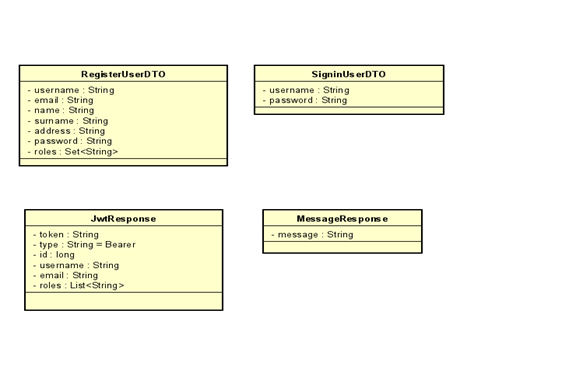
\includegraphics[scale=1]{slike/DijagramRazredaD.PNG} %veličina slike u odnosu na originalnu datoteku i pozicija slike
				\centering
				\caption{Dijagram razreda - DTO}
				\label{fig:dijagramRazredaC}
			\end{figure}
	
	
			\begin{figure}[H]
				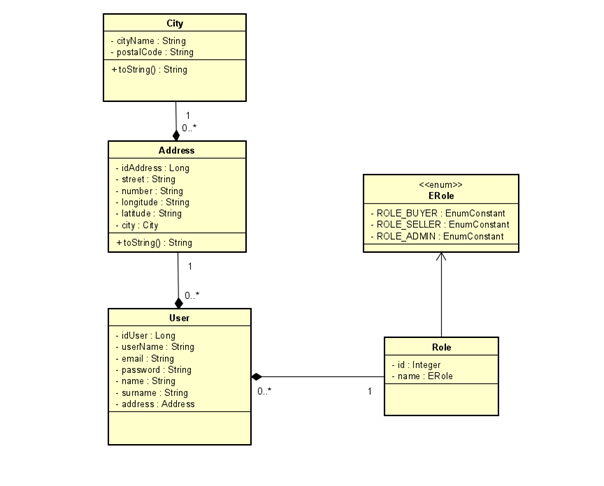
\includegraphics[scale=1]{slike/DijagramRazredaM.PNG} %veličina slike u odnosu na originalnu datoteku i pozicija slike
				\centering
				\caption{Dijagram razreda - Models}
				\label{fig:dijagramRazredaC}
			\end{figure}
			
			\eject
		
